

\section{Anharmonic effects in thermal conduction}

\subsection{Interfacial thermal conductance (\citepub{spectral})}

\begin{figure}[tb]
 \begin{center}
  %\includegraphics[width=.99\columnwidth]{/Users/saaskilak/Documents/matlab/pics/171213a_cnt.ps}
 % \includegraphics[width=.99\columnwidth]{/Users/saaskilak/Documents/latex/pics/240114_fcc_final.ps}
  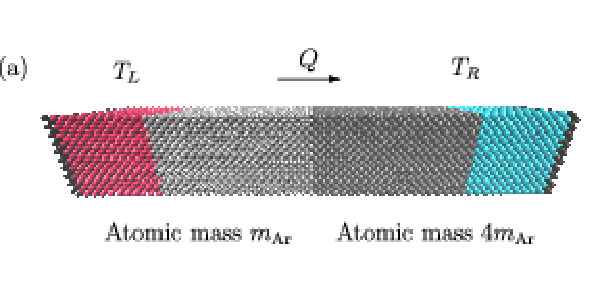
\includegraphics[width=8.6cm]{pics/nemd_fig2a.pdf}
  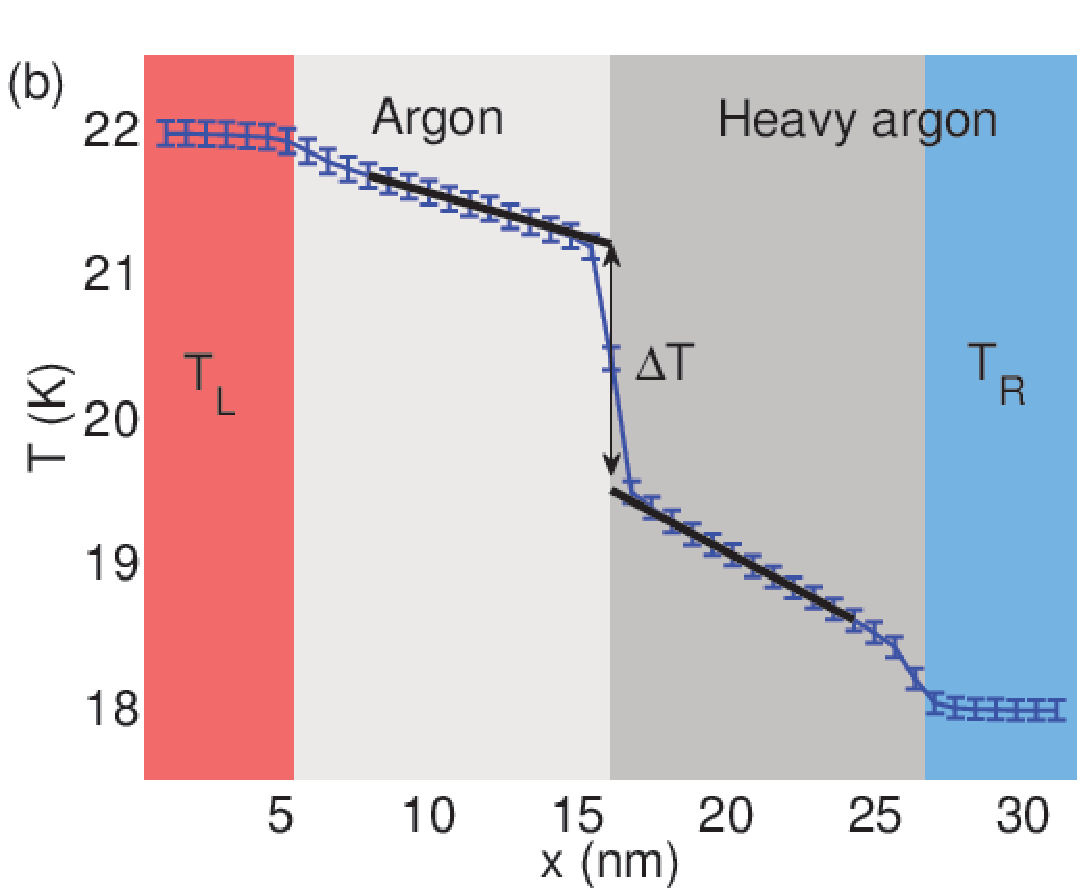
\includegraphics[width=8.6cm]{pics/nemd_fig2b.pdf}
  \caption{(a) Atomistic illustration of the studied interface between two mass-mismatched Lennard-Jones solids. The atoms at the left and right ends are coupled to Langevin heat baths at different temperatures $T_L$ and $T_R$ to drive thermal current $Q$ through the interface in the middle. (b) Local kinetic temperature profile in a non-equilibrium simulation with average temperature $T=20$ K. Temperature drop $\Delta T$ at the interface is estimated by extrapolating the linear fits to the temperature profiles at different sides of the interface and calculating the difference at the interface. } 
 \label{fig:nemd_fig1}
 \end{center}
\end{figure}

\begin{figure}[tb]
 \begin{center}
  %\includegraphics[width=.99\columnwidth]{/Users/saaskilak/Documents/matlab/pics/171213a_cnt.ps}
 % \includegraphics[width=.99\columnwidth]{/Users/saaskilak/Documents/latex/pics/240114_fcc_final.ps}
  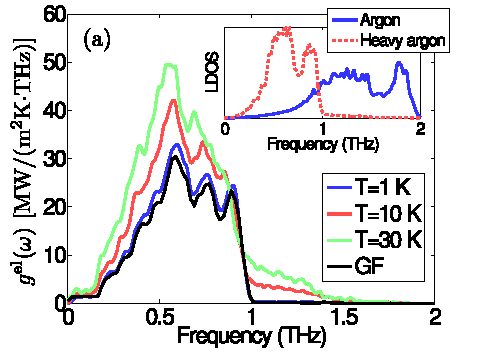
\includegraphics[width=.49\columnwidth]{pics/nemd_fig4a.pdf}
  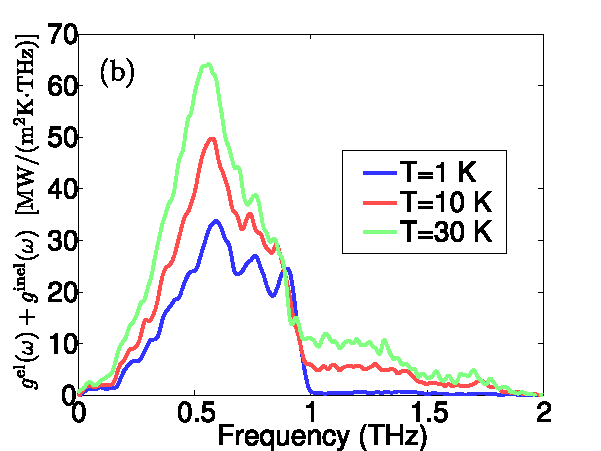
\includegraphics[width=.49\columnwidth]{pics/nemd_fig4b.pdf}
  \caption{The elastic conductance  \eqref{eq:gel} as a function of frequency at various temperatures. At $T=1$ K, the elastic conductance agrees very well with the Landauer-B\"uttiker conductance $g^{\textrm{LB}} (\omega)=k_B \mathcal{T}(\omega)/A$, where the transmission function $\mathcal{T}(\omega)$ has been calculated for the interface between two semi-infinite LJ solids using the Green's function (GF) method. At high temperatures, inelastic effects in the bulk enable energy transmission also above the cut-off frequency $f_c^{(2)}=1$ THz of the heavier solid. Inset: Local density of vibrational states (LDOS, arbitrary units) at the interface calculated from MD at $T=1$ K. In the lighter solid with mass $m_1=m_{\textrm{Ar}}$ (argon, solid line), vibration frequency cut-off is $f_c^{(1)}=2$ THz. In the heavier medium with mass $m_2=4m_1$ (heavy argon, dashed line), bulk vibrations therefore only extend up to $f_c^{(2)}=1$ THz, limiting ballistic transmission of phonons below this limit. At the interface, however, there are evanescent wave states extending up to 1.5 THz. (b) The sum $g^{\textrm{el}}(\omega)+ g^{\textrm{inel}}(\omega)$ of elastic and inelastic [Eq. \eqref{eq:ginel_dec}] spectral conductance as a function of frequency. At high temperatures, the inelastic energy transfer processes strongly enhance interfacial heat transfer at $f\approx 0.5$ THz and above the cut-off $f_c^{(2)}=1$ THz.} 
 \label{fig:nemd_fig2}
 \end{center}
\end{figure}

\subsection{Mean free paths (\citepub{cnt})}

\begin{figure}[tb]
 \begin{center}
  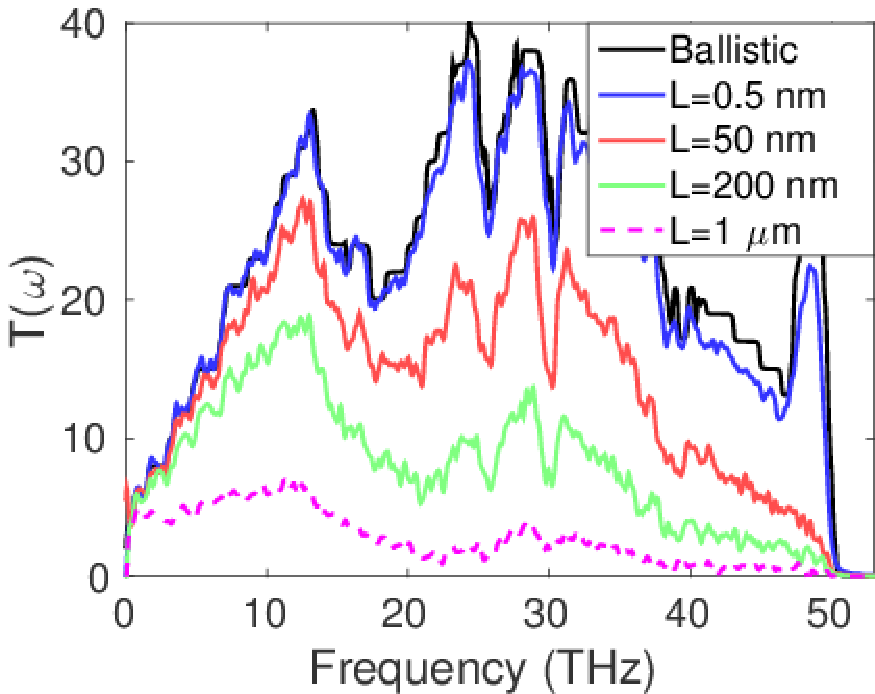
\includegraphics[width=.49\columnwidth]{pics/cnt_fig2.pdf} 
  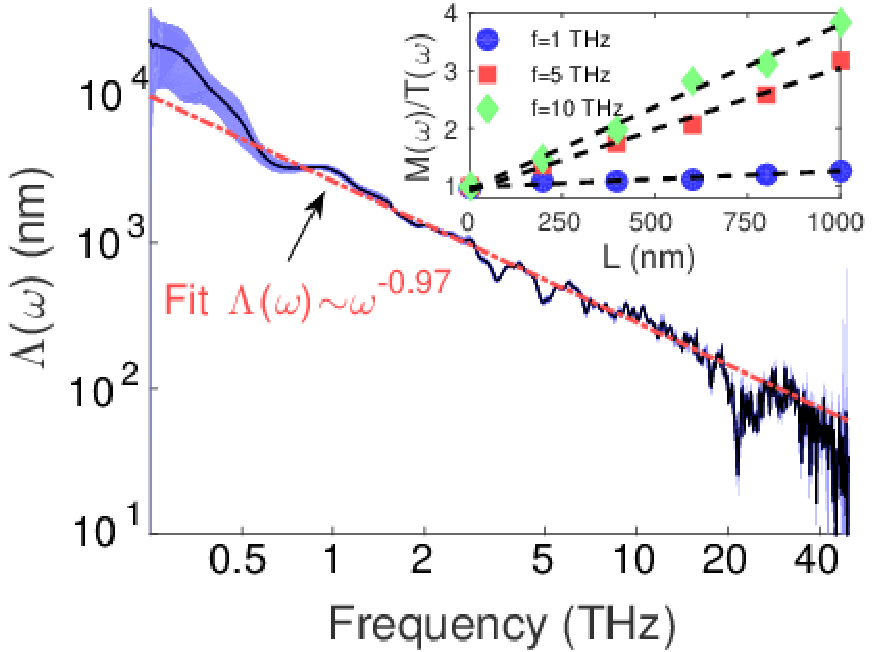
\includegraphics[width=.49\columnwidth]{pics/cnt_fig4.pdf} 
  \caption{(a) Spectral transmission function $\ca{T}(\omega)=q(\omega)/(k_B\Delta T)$ for various tube lengths at $T=300$ K, determined from the NEMD simulations. As expected, increasing the tube length reduces the transmission. For $L=0.5$ nm, the spectral conductance is very close to the ballistic value $M(\omega)$ determined by counting the number of propagating modes from the phonon bandstructure of Fig. \ref{fig:bs}. (b) Log-log plot of the mean free path $\Lambda(\omega)$ at $T=300$ K. The inset shows the scaled inverse transmission functions $M(\omega)/\ca{T}(\omega)$ as a function of tube length $L$. The mean free paths are determined from the inverse slopes of the least-square linear fits (dashed, black lines in the inset) calculated using an automated numerical routine at each frequency. The shaded regions in the main figure correspond to the 92.5\% confidence interval for the slope. Below 0.25 THz, the confidence interval is very large (not shown) due to numerical uncertainties, inhibiting the reliable determination of mean free paths for very small frequencies.}  
\label{fig:cnt_fig2}
 \end{center}
\end{figure}

\section{Interference effects in constrictions (Publications \cp{fpu}, \cp{fpu2})}

\begin{figure}
\begin{center}
 %\includegraphics[width=8.6cm]{../scbaths_paper_re_resubmission/pic1.ps}
 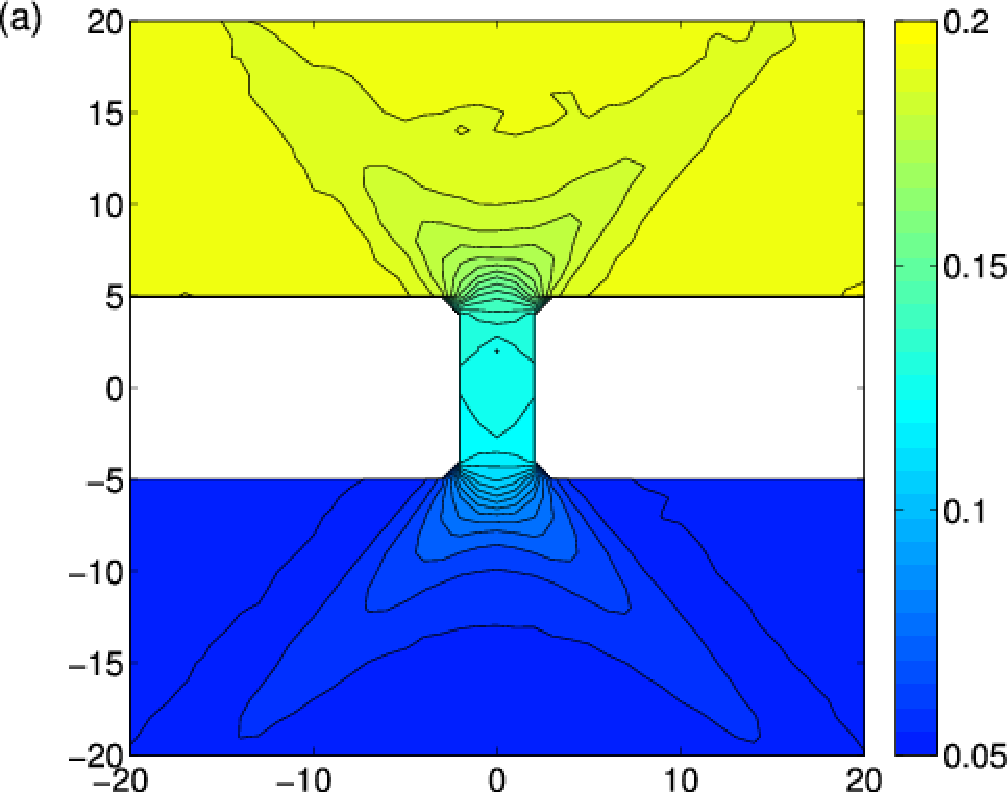
\includegraphics[width=.49\columnwidth]{pics/fpu_fig2a.pdf}
  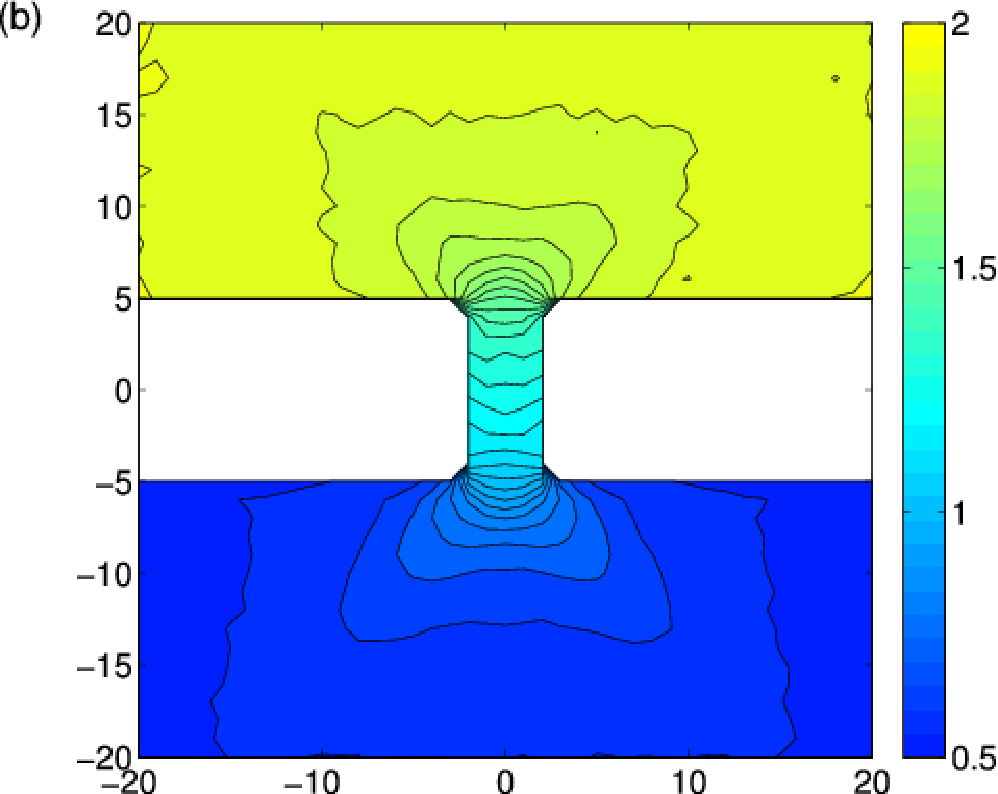
\includegraphics[width=.49\columnwidth]{pics/fpu_fig2b.pdf}
 \caption{Kinetic temperature profile at (a) low temperature ($T_+=0.20$, $T_-=0.05$) and (b) high temperature ($T_+=2.0$, $T_-=0.5$). The bulk size is $W^R=161$, $L^R=80$ and the constriction size $W^C=5$, $L^C=9$. The labels on the horizontal and vertical axes mark the atom indices. The separations of isolines are (a) $0.005$ and (b) $0.05$.}
\label{fig:fpu_fig2}
\end{center}
\end{figure}

\begin{figure}
\begin{center}
 %\includegraphics[width=8.6cm]{../scbaths_paper_re_resubmission/pic1.ps}
 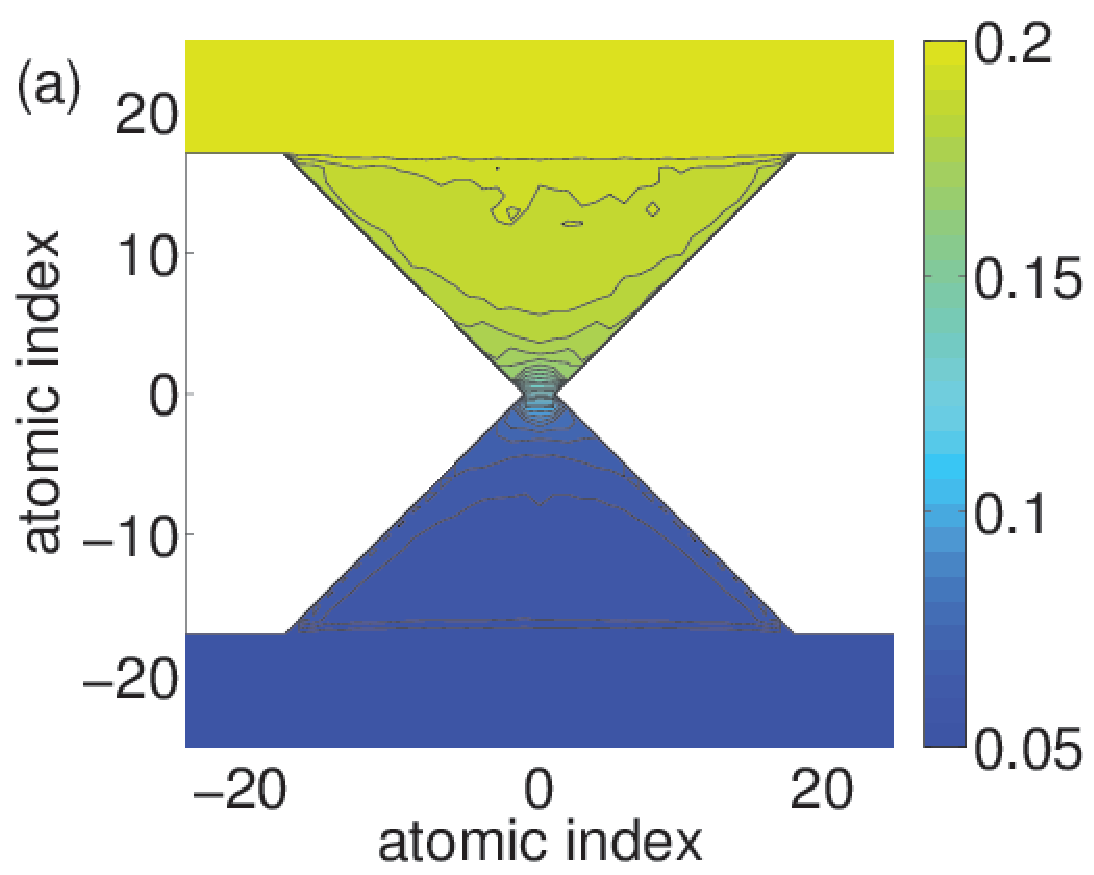
\includegraphics[width=.49\columnwidth]{pics/aip_fig5a.pdf}
 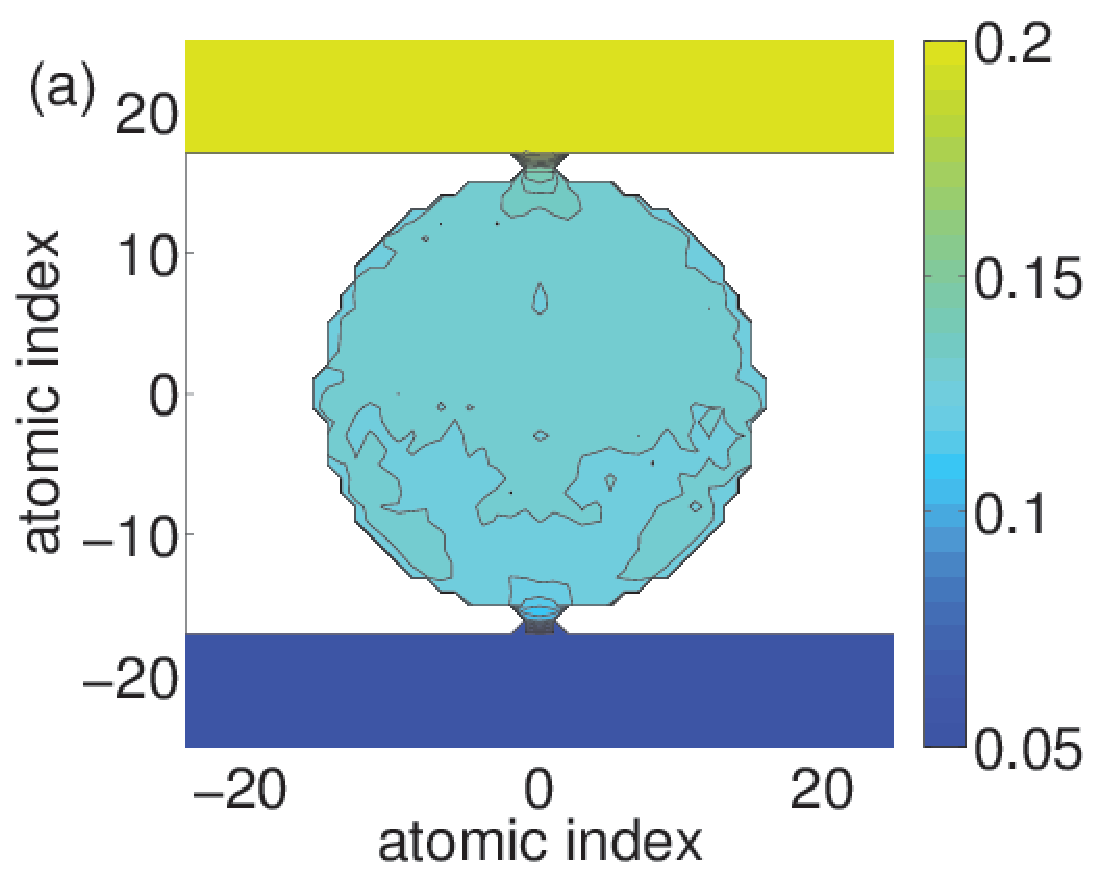
\includegraphics[width=.49\columnwidth]{pics/aip_fig6a.pdf}
 %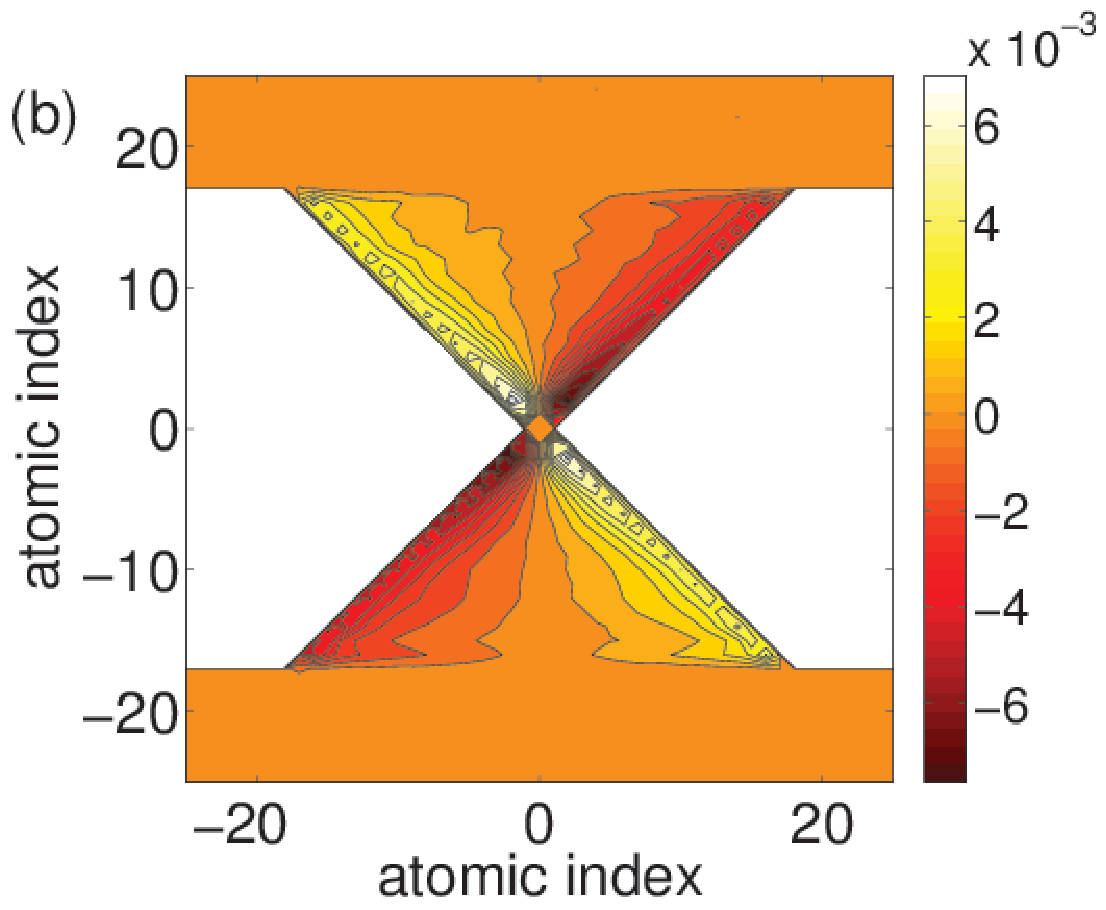
\includegraphics[width=.49\columnwidth]{pics/aip_fig5b.pdf}
 \caption{Kinetic temperature profile in (a) triangular constriction (b) discoid constriction. The separations of isolines are (a) and (b) .}
\label{fig:aip_figs56}
\end{center}
\end{figure}

\section{Langevin models of lattice and electromagnetic energy transfer}

\subsection{Quantum effects in constrictions (\citepub{gf}): Self-consistent heat bath model}

\label{sec:results_schb}
Let us now present an application for the linearized Langevin equations presented above. For vibrational heat transfer, employing the linearized Langevin equations \eqref{eq:th_eom1} leads to the self-consistent heat bath model \cite{bolsterli70}. Whereas earlier works have applied the model to simple one-dimensional systems (see, e.g., Refs. \cite{bolsterli70,visscher75,dhar03,dhar06,segal09,bandyopadhyay11}) with a finite number of atoms, \citepub{gf} extended the model to more complex geometries with an infinite number of atoms.  %The model was then applied to investigating quantum temperature profiles in constrictions in rectangular lattices and graphene.

% An exemplary computational setup for vibrational heat transfer modeling is illustrated in Fig. \ref{fig:schb_setup} for a constriction in a two-dimensional lattice, studied in \citepub{gf}. Similar configuration was also applied to one-dimensional chains and a point contact in graphene in the same publication. 

\begin{figure}
\begin{center}
 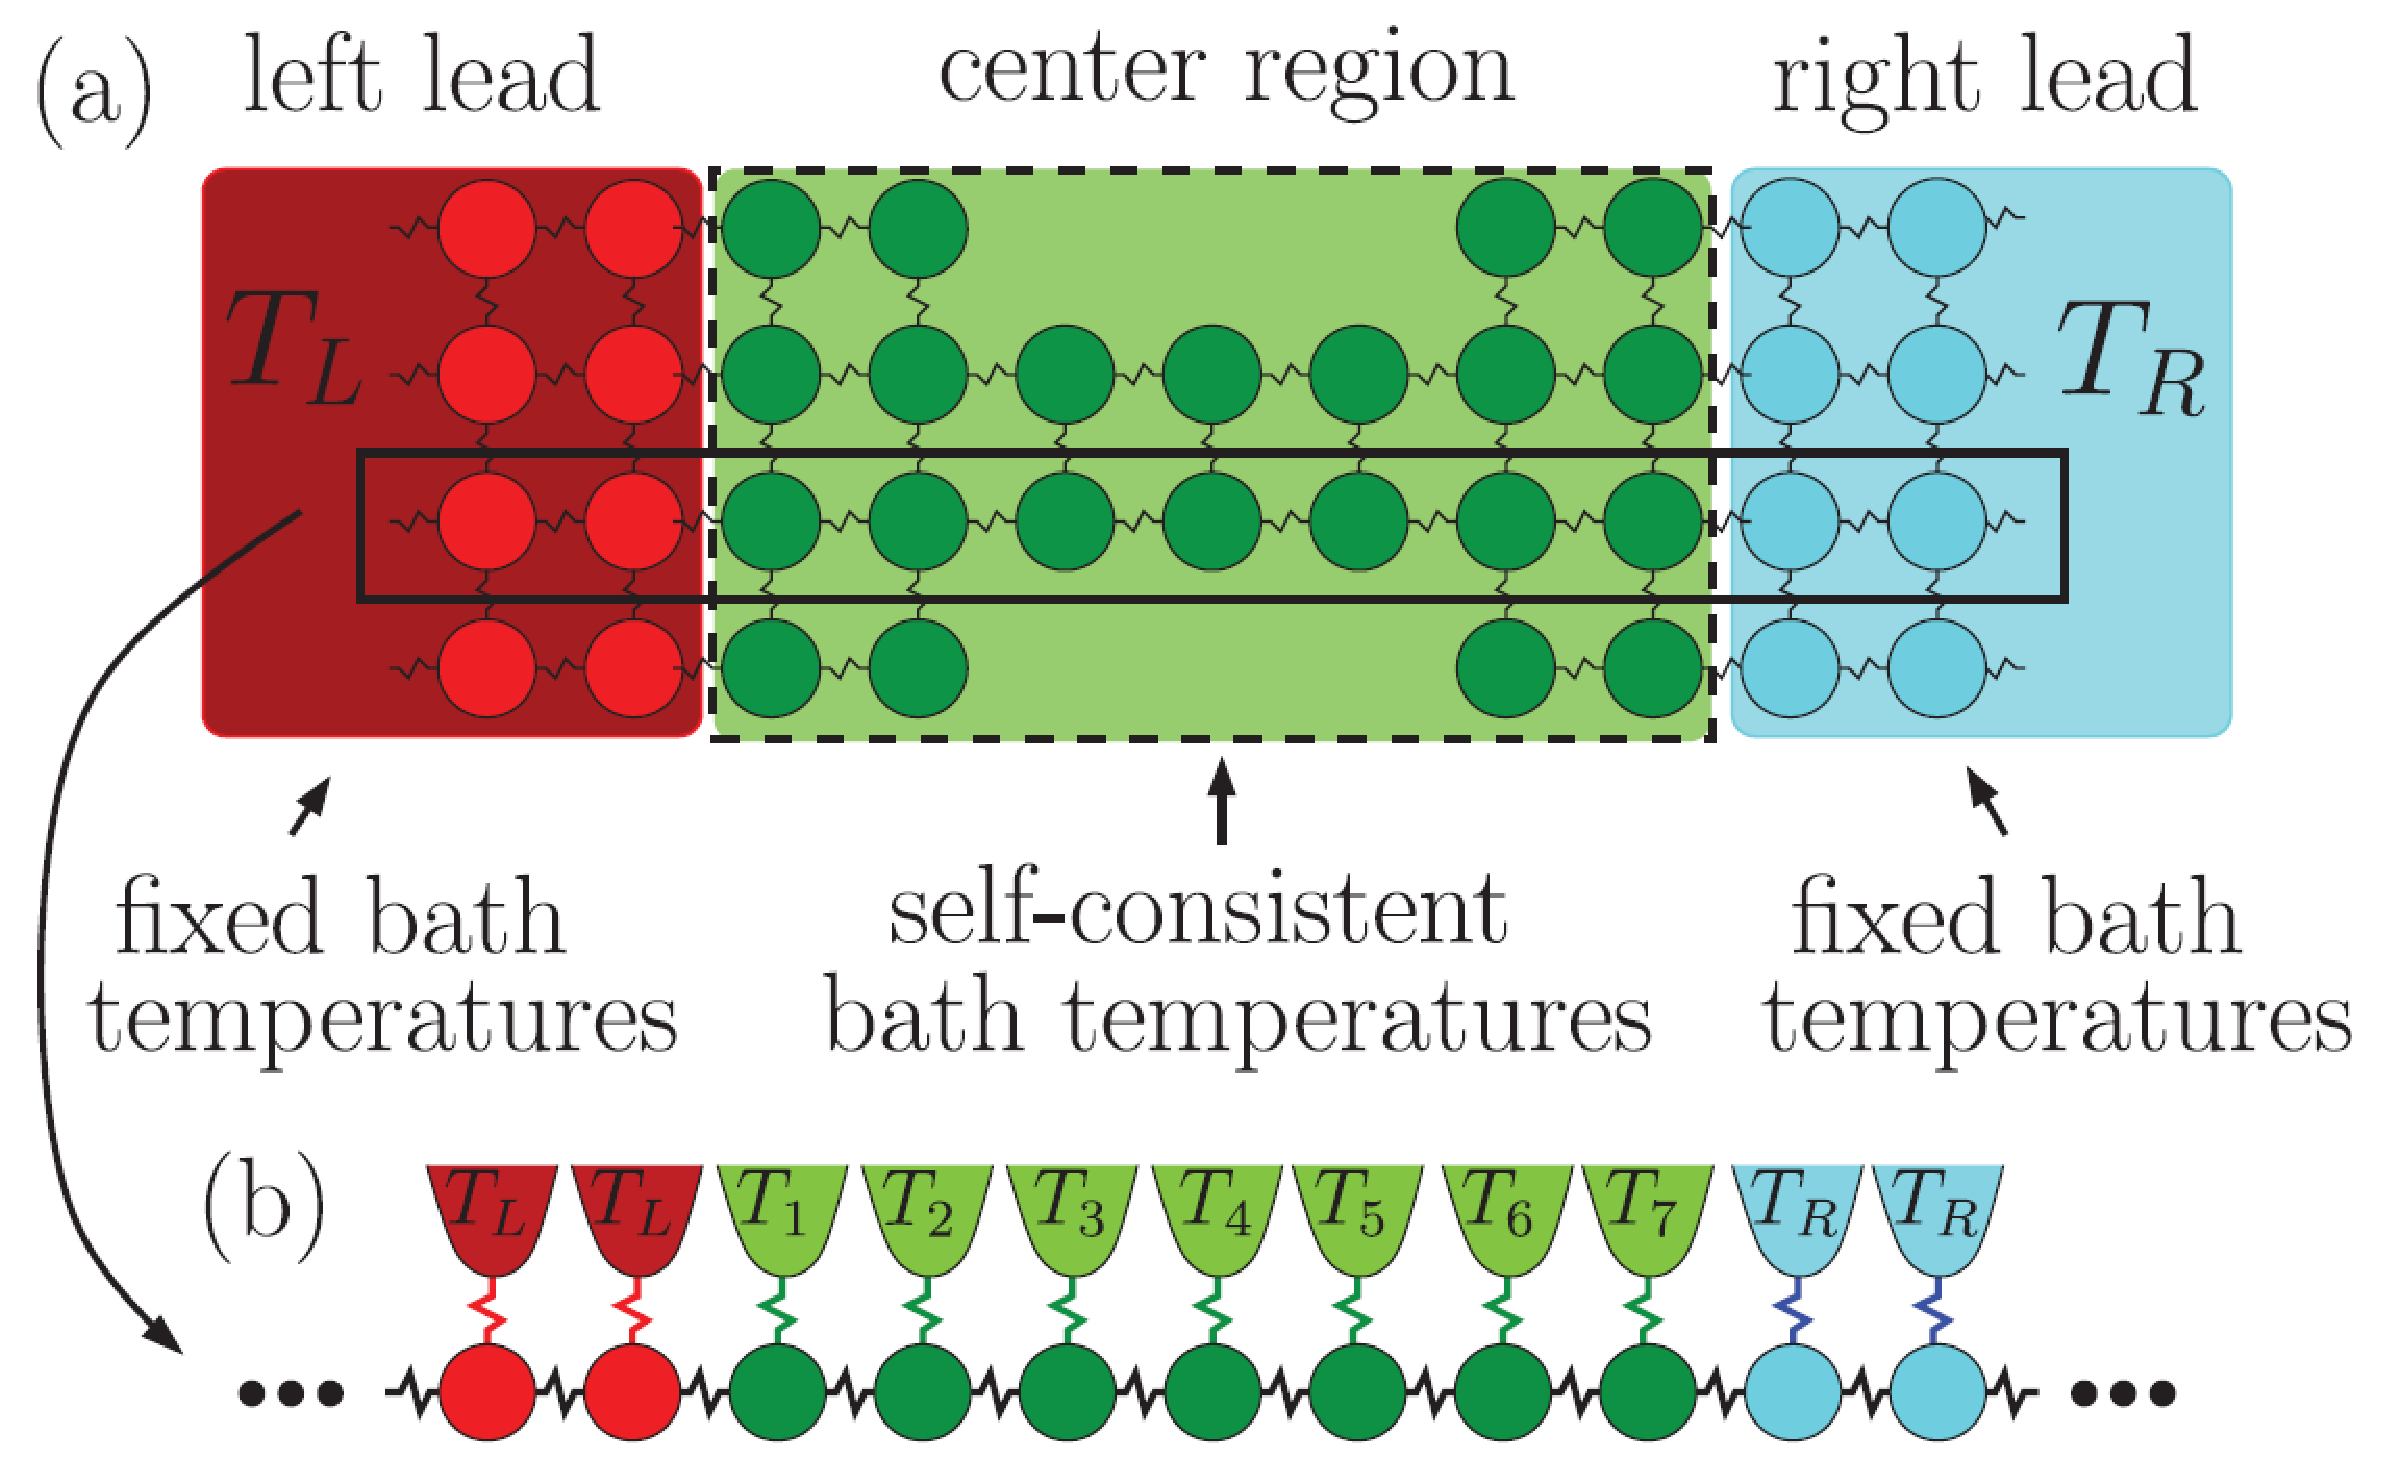
\includegraphics[width=.99\columnwidth]{pics/schb_setup.pdf}
 \caption{A schematic illustration of the self-consistent heat bath model for a constriction in a two-dimensional rectangular lattice. The system consists of the left lead, the center region, and the right lead. All atoms are coupled to Langevin heat baths explicitly for one cross section in (b). Whereas the temperatures of the Langevin baths have prescribed values $T_L$ and $T_R$ in the left and right lead, temperature varies between $T_L$ and $T_R$ in the center region. Following the self-consistent bath model \cite{bolsterli70}, the bath temperatures are determined self-consistently in the center region from the requirement that the thermal current to each bath is zero. Reprinted from \citepub{gf} with publisher's permission.}
\label{fig:schb_setup}
\end{center}
\end{figure} 

The setup of \citepub{gf} is schematically illustrated in Fig. \ref{fig:schb_setup}. The setup consists of a center region with a finite number of atoms and left and right leads with possibly an infinite number of atoms. All atoms are coupled to local Langevin baths mimicking all interaction events driving the system towards local thermal equilibrium \cite{bolsterli70}. In the center region of Fig. \ref{fig:schb_setup}(a), a constriction acts as a scattering center for phonons coming in from the left and right leads. Around the constriction, bath temperatures are unknown, so they are determined self-consistently from the requirement that the heat current to each bath vanishes \cite{bolsterli70}. The requirement of zero heat current to local baths ensures that the heat current flowing in the chain is conserved at each atom site, a natural requirement in the steady-state. Away from the scattering region, the baths are set to prescribed temperatures $T_L$ and $T_R$. The modeling of atomic dynamics in the leads by Langevin terms contrasts with earlier works \cite{dhar06} and enables perfect acoustic matching between the leads and the center region, as discussed in \citepub{gf}.  % The baths then act as quantum-mechanical temperature probes. 

% \begin{figure}
% \begin{center}
%  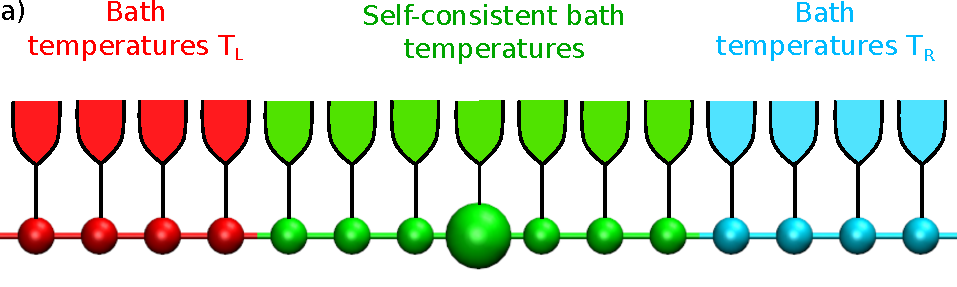
\includegraphics[width=.99\columnwidth]{pics/chain_rg.pdf}
%   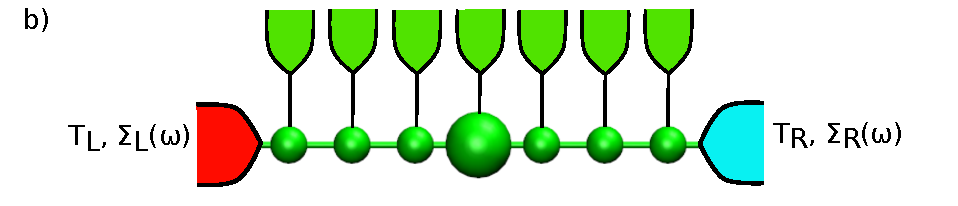
\includegraphics[width=.99\columnwidth]{pics/chain_rg2.pdf}
%  \caption{(a) Schematic illustration of the self-consistent bath model for an atomic chain with a mass defect. In the neighborhood of the mass defect acting as a scattering center, the bath temperatures are determined self-consistently from the requirement of vanishing heat current to the baths. In the left and right leads (red and blue, respectively), the bath temperatures are fixed at $T_L$ and $T_R$. (b) Illustration of the replacement of the leads by single Langevin heat baths at temperatures $T_L$ and $T_R$. The details of lattice dynamics in the leads is fully captured by the self-energy matrices $\Sigma^L(\omega)$ and $\Sigma^R(\omega)$, defined in detail in \citepub{gf}.}
% \label{fig:chain_rg}
% \end{center}
% \end{figure} 


The calculation of heat currents starts from writing down the Langevin equation of motion \eqref{eq:th_eom1} for each atom $i$ with interatomic force constants $\bb{K}_{ij}$ determined from interatomic potential energy as discussed in Sec. \ref{sec:th_eom2_phonon}. The relaxation rate $\gamma$ is chosen to correspond to known phonon life-times. As shown in \citepub{gf}, solving the equations of motion for the leads and substituting to the equations for the center region allows for replacing the leads by \textit{single} Langevin heat baths at temperatures $T_L$ and $T_R$, which reduces the number of degrees of freedom to those in the center region. The microscopic details of lattice dynamics in the leads are fully captured by the lead self-energy functions $\Sigma^L(\omega)$ and $\Sigma^R(\omega)$. Microscopic definitions of the self-energy function in terms of the lead Green's function and the fluctuation-dissipation theorem for the corresponding Langevin noises are presented in detail in \citepub{gf}.



% The self-consistent bath model can be similarly extended for complex electron systems to study local heating and thermoelectric effects in quantum transport \cite{roy07}. 
% The heat current to each local bath at site $i$ can be determined by calculating the rate of change of local energy \cite{hardy63}, which reads in the harmonic approximation
% \begin{equation}
%  e_i = \frac{1}{2}m\dot{\bu}_i^2 + \frac{1}{2} \sum_{\alpha,\beta}\sum_j u_i^{\alpha} K_{ij}^{\alpha\beta} u_j^{\beta} . \label{eq:th_ei}
% \end{equation}
% Calculating the time derivative of Eq. \eqref{eq:th_ei} and thermal averaging gives
% \begin{equation}
%  \langle \dot{e}_i \rangle = -\sum_j  J_{ij} -  Q_i ,
% \end{equation}
% where the first term in brackets on the right hand side corresponds to the heat current
% \begin{equation}
%  J_{ij} = \frac{1}{2} \sum_{\alpha,\beta} \left\langle \dot{u}_i^{\alpha}K_{ij}^{\alpha\beta} u_j^{\beta} - u_i^{\alpha} K_{ij}^{\alpha\beta} \dot{u}_j^{\beta} \right\rangle
% \end{equation}
% between particles $i$ and $j$ and the second term is the heat flow to the bath, defined as 
% \begin{equation}
%  Q_i = \langle [m\gamma \dot{\bu}_i-\xi_i] \cdot \bu_i \rangle.
% \end{equation}


Evaluation of heat currents flowing to baths in terms of the center region's Green's function $\bb{G}(\omega)$ leads to the Landauer-B\"uttiker-like expression \eqref{eq:th_QI}, where the bath indices $I$ and $J$ correspond to local baths in the center region and the two leads. This calculation is outlined in Sec. \ref{sec:th_currents} and carried out in detail in \citepub{gf}. %The transmission function is given by Eq. \eqref{eq:th_caroli} and $\Gamma^I(\omega)=-2\textrm{Im}[\Sigma^I(\omega)]$ is the bath coupling function, as again explained in \citepub{gf}.

By setting Eq. \eqref{eq:th_QI} equal to zero for the local baths in the center region, one gets a non-linear system of equations for the bath temperatures. This system of equations can be solved by, e.g., using Newton-Raphson method \cite{bandyopadhyay11} or resorting to linearizing approximations \cite{segal09}. The self-consistent temperature profile and the evaluation of heat currents flowing to the two leads then constitute a solution of the vibrational heat transfer problem. Results for constrictions in two-dimensional lattices are presented in Sec. \ref{sec:results_gf}.

The same principles as outlined here for phonon transport can be directly applied to electron transport as well, when Langevin heat baths are replaced by electron baths. In this case, the self-consistent baths are often referred to as voltage-temperature probes \cite{jacquet09}. Applications of voltage-temperature probe models for describing dissipation effects in electron transport have been so far limited only to one-dimensional geometries \cite{buttiker86,damato90,jacquet09,jacquet12}, although the model can account for wave dynamics, Joule heating as well as thermoelectric effects \cite{roy07}. Recently, Bergfield \textit{et al.} used the model for investigating quantum temperature oscillations in graphene \cite{bergfield15}.

%The similarities of the equations of motion become more apparent in the linear approximation, which is discussed in more detail below. In this case, the force acting on atom $i$ becomes $F_i^{\alpha}=-\sum_{j}\sum_{\beta} K_{ij}^{\alpha\beta}u_j^{\beta}$ and the electron Hamiltonian 

% \subsubsection{Electromagnetic energy transfer in a cavity}

\begin{figure}
 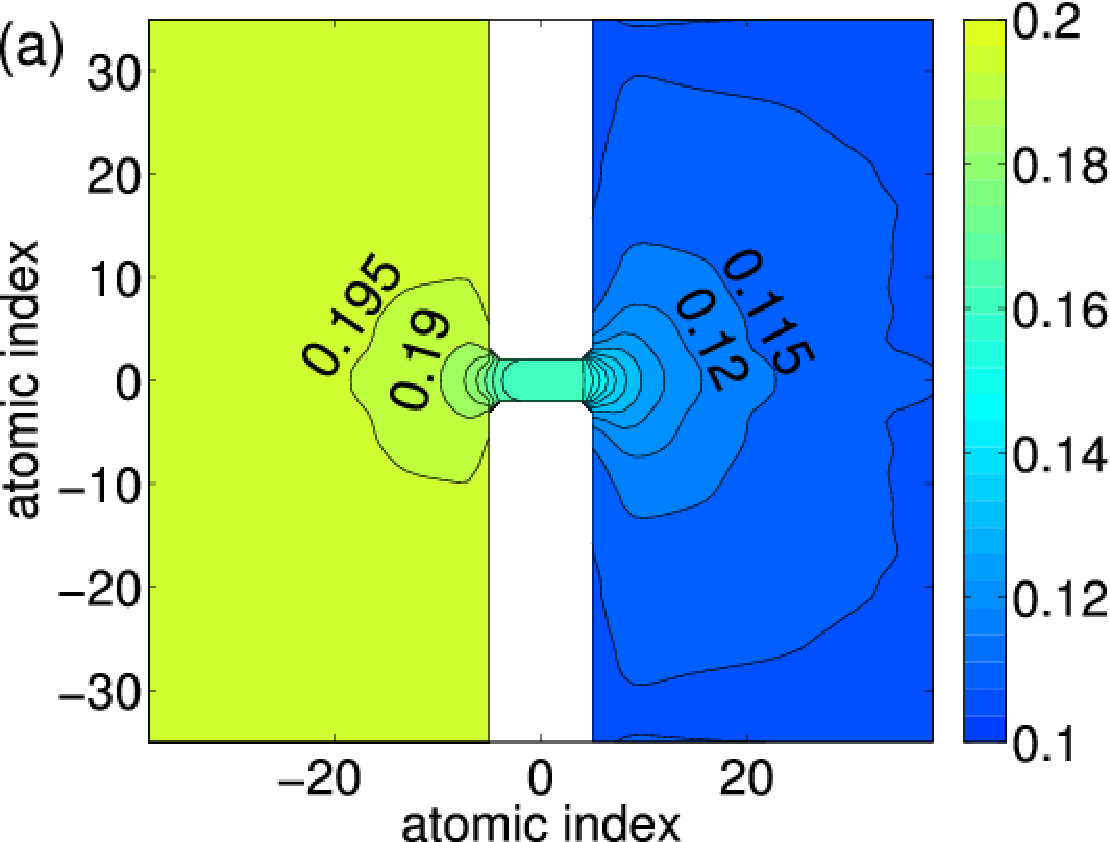
\includegraphics[width=.49\columnwidth]{pics/gf_fig7a.pdf}
 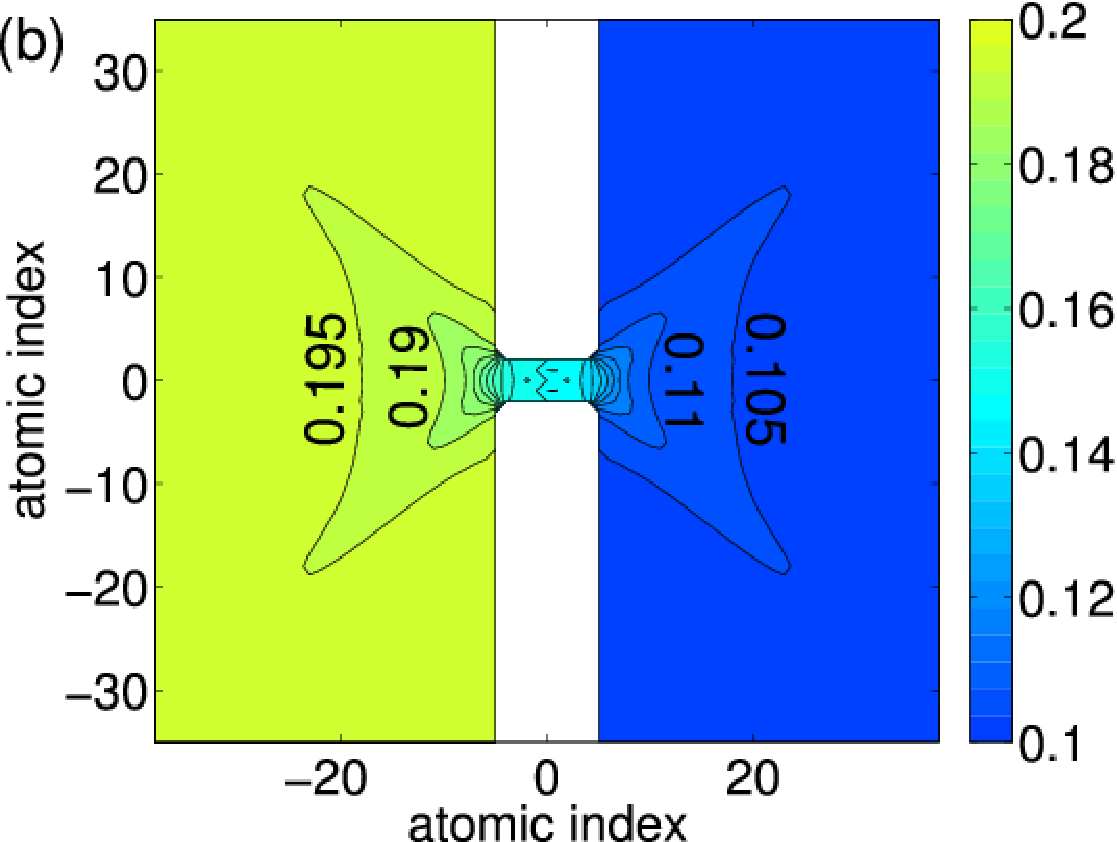
\includegraphics[width=.49\columnwidth]{pics/gf_fig7b.pdf}
 \caption{Bath temperature profiles in a $w=5$, $l=9$ constriction coupled to leads of width $W=71$ and $L=35$ [see Fig. \ref{fig:chain_rg}(b)]. Lead temperatures are $T_L=0.2$ and $T_R=0.1$. Figures show (a) quantum exact and (b) classical self-consistent bath temperature profiles. Friction parameter is $\gamma=0.01$. The separation of isolines is $0.05$ and four contour lines are labeled for convenience.}
 \label{fig:gf_fig7}
\end{figure}

\begin{figure}
 \begin{center}
 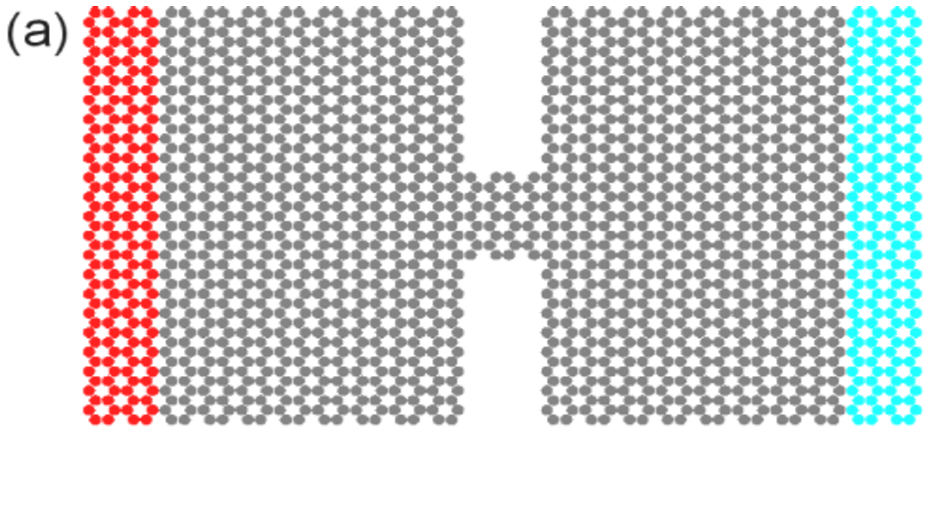
\includegraphics[width=.49\columnwidth]{pics/gf_fig8a.pdf}
 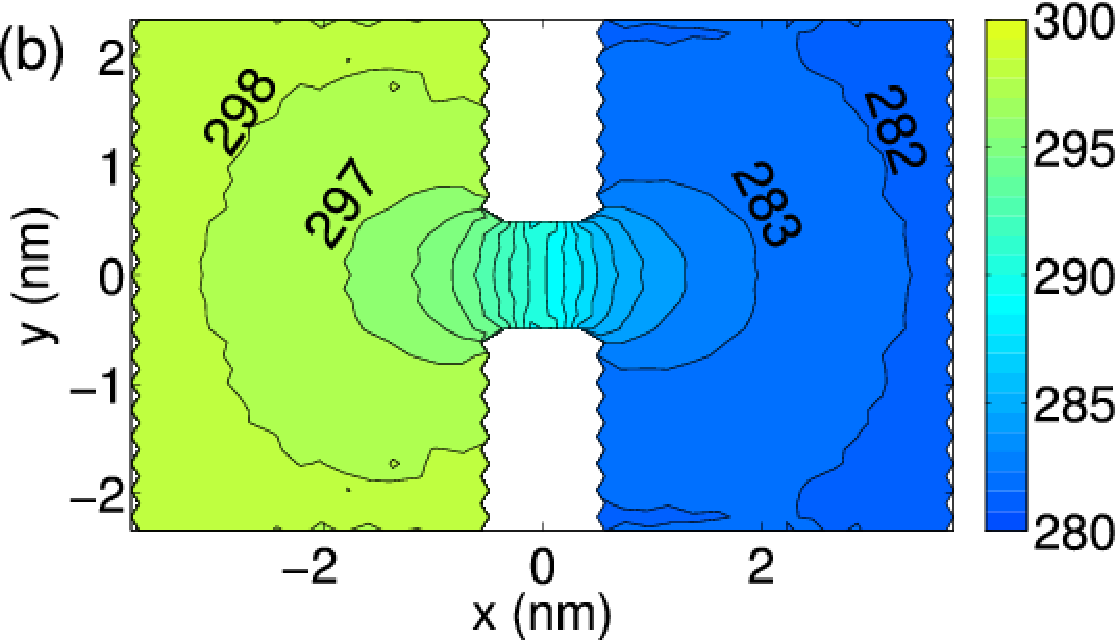
\includegraphics[width=.49\columnwidth]{pics/gf_fig8b.pdf}
 \end{center}
 \caption{(a) Graphene nanoconstriction. The leads extend infinitely to the left and right, but the temperatures are determined self-consistently only for the gray atoms in the shown center region. (b) Self-consistent bath temperature profiles (K). The semi-infinite leads are at temperatures $T_L=300$ K and $T_R=280$ K. The relaxation time $\tau=1/\gamma$ is set to $1$ ps.}
 \label{fig:gf_fig8}
\end{figure}

\subsection{Cavity-modified electromagnetic energy transfer (\citepub{dipole})}





\begin{figure}[tb]
 \begin{center}
  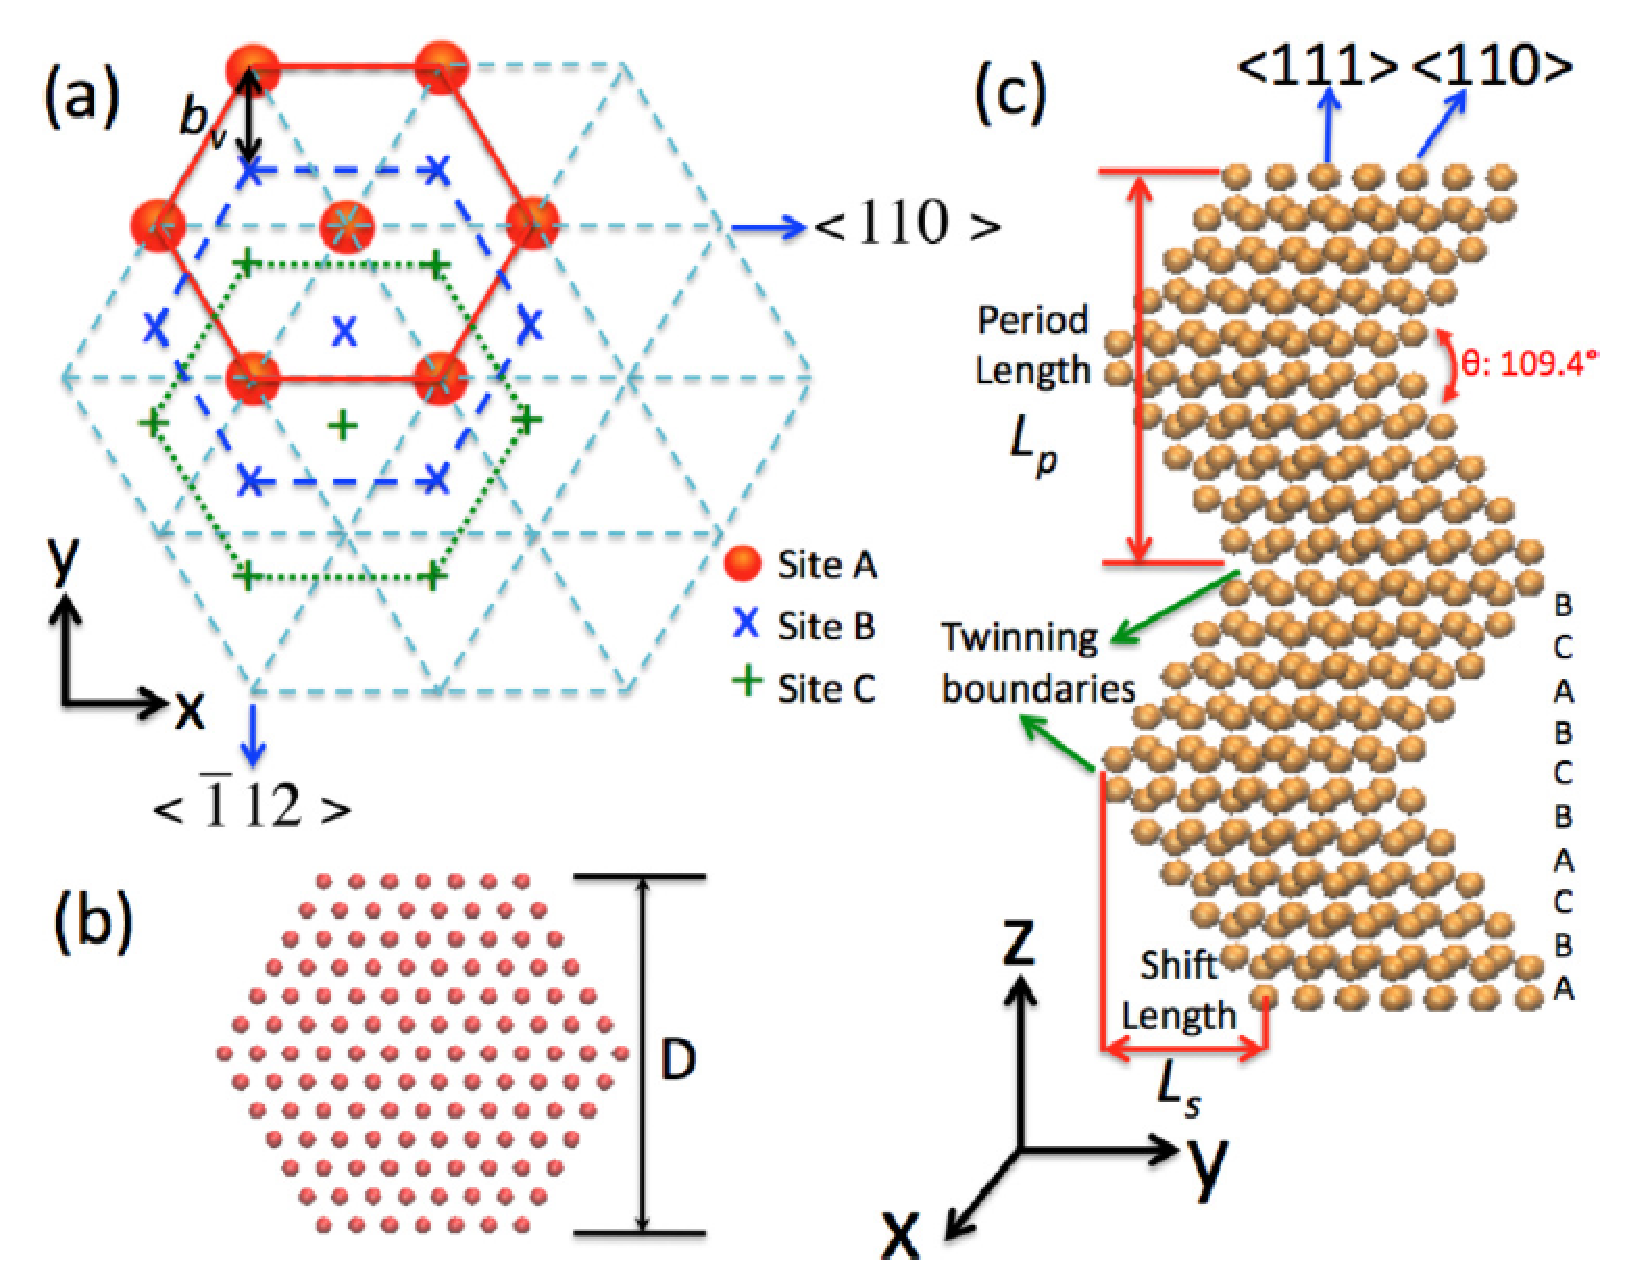
\includegraphics[width=.49\columnwidth]{pics/twinning_fig1.pdf} 
  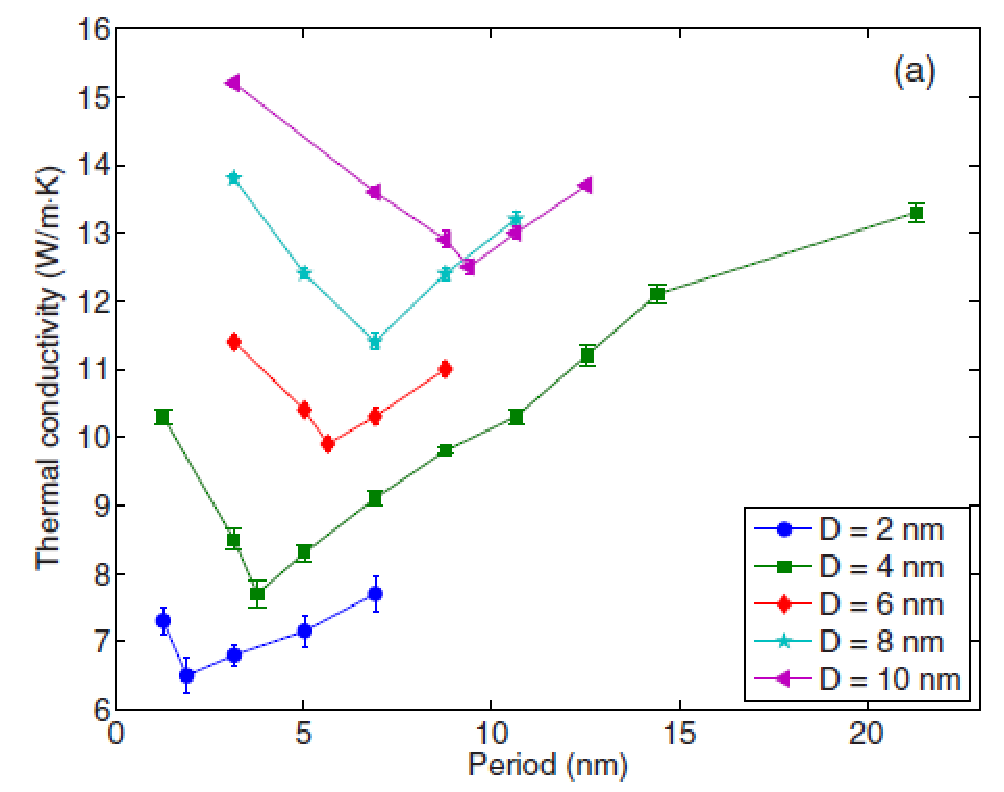
\includegraphics[width=.49\columnwidth]{pics/twinning_fig2a.pdf} 
  \caption{}  
\label{fig:twinning_fig1}
 \end{center}
\end{figure}

